\section{Component Tools for Reproducible Research}


\section{Measuring Dependencies}

\begin{figure*}
\centering
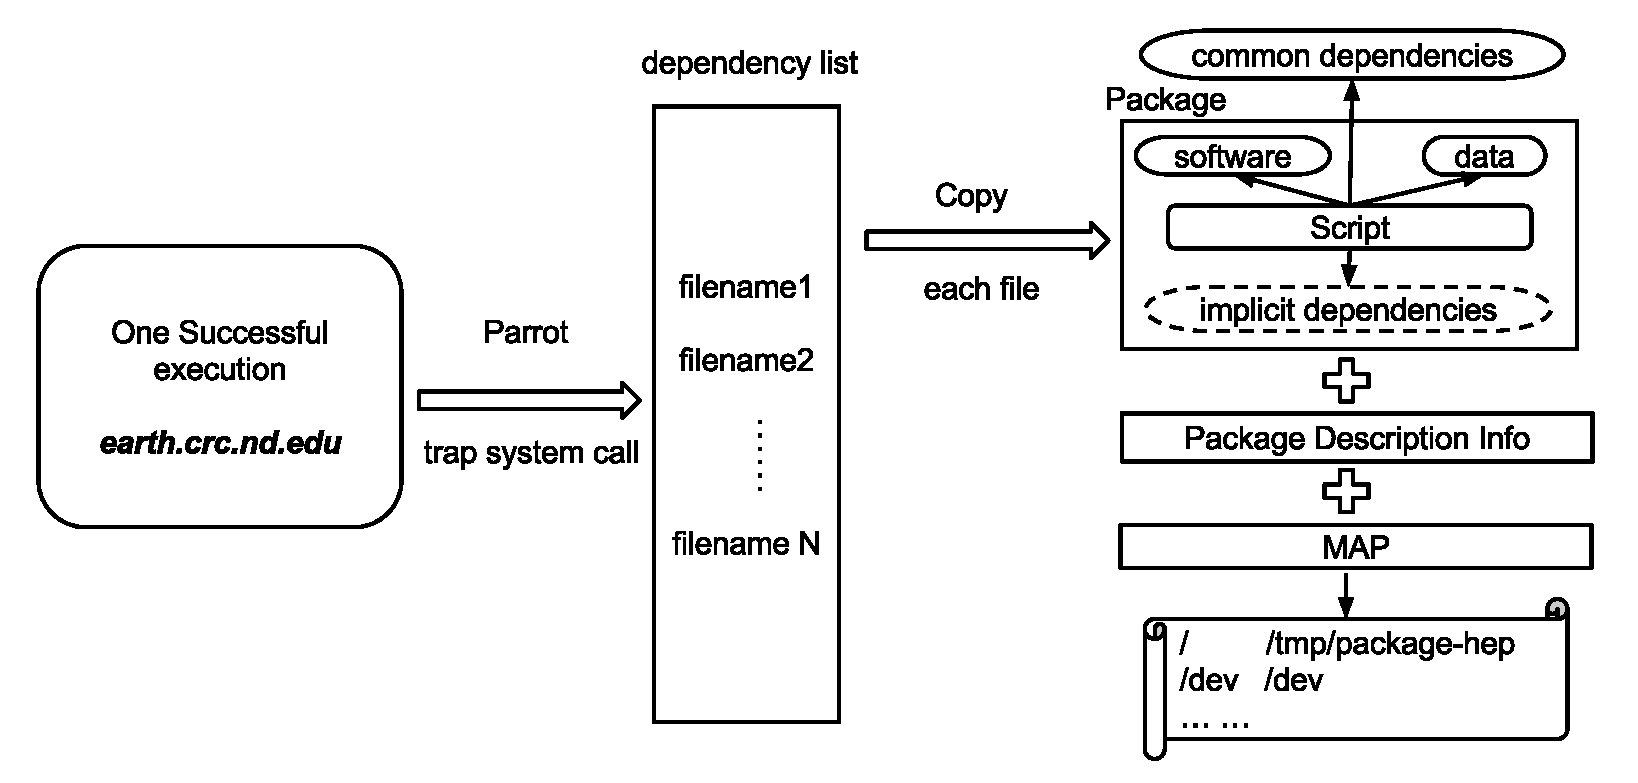
\includegraphics[width=.8\textwidth]{workflow-parrot.eps}
\caption{Workflow of The Fine-Grained Dependency Management Toolkit Based on Parrot}
\label{fig:workflow-parrot}
\end{figure*}

We have developed a prototype tool to assist in the measurement and preservation
of implicit dependencies for complex applications.
We use Parrot~\cite{thain2005parrot} to explicitly record all
of the files accessed by our example application, allowing us to observe how
much of each external dependencies is used, and what local resources are implicitly used.
Using this information, we create a \emph{reduced package} which contains
only the files actually used by the application.

Parrot is a virtual filesystem access tool which has been used to attach
existing programs to a variety of remote I/O systems, such as HTTP, FTP, and CVMFS.
It works by trapping an application's system calls through the Linux {\tt ptrace} debugging
interface, and then replacing them with the desired I/O operations.  Parrot is already used
in the high energy physics community with applications like TauRoast specifically to 
provide access to the CMSSW software distribution via the CVMFS distributed file system.
We made small modifications to Parrot to record a \emph{namelist} which lists all 
of the files that an application actually accesses.

Figure~\ref{fig:workflow-parrot} illustrates the measurement process.
The starting point of this toolkit is one successful execution of the application on the native machine.
First, we execute the actual data analysis script under Parrot to generate the namelist.
Then, using the namelist, we generate a package containing all the necessary data
and software for one analysis program. When another
researcher wants to repeat the program, he only needs to obtain the package and
execute the actual analysis program inside the package. 

For one execution of \emph{TauRoast}, the generated namelist includes 132,047 accessed filenames,
along with the system calls used to access the file, such as {\tt open}, {\tt stat}, {\tt read}, etc.
With duplicate filenames removed, the list is reduced to 67,168 files.
Many of those entries do not exist, because they reflect attempts
by the application to search for programs and libraries in multiple places.
Only 22,068 entries reflect existing files or directories.

The packaging tool iterates over each item of the filename list, determines the process
mode and replication degree according to the file type (common files,
directories, symbolic links) and the system call type, generates one package
containing the dependencies, and summarizes the contents of the package
as shown in Table~\ref{table:package-info}.  To the extent possible,
the filesystem structure of the original environment is preserved.

We considered several approaches to constructing the package.
In a {\bf shallow copy}, we only copied the individual files in the namelist,
creating only parent directories for each.  Where a directory was listed,
we created the directory and populated it with empty files as placeholders
to facilitate a directory listing.  In a {\bf medium copy}, we copied the
individual files as before.  Where a directory was listed, we created
the directories and copied the contents of the files in that directory,
one level deep.  A {\bf deep copy} would duplicate all directories recursively,
but this would have resulted in TB-sized packages, so we did not consider
it further.

Parrot is required to re-run the packaged artifact, in order to force
the packaged files to appear to exist in their original locations.
To this end, the packaging tool creates a \emph{file map} which maps
the logical names of the files to their current physical locations, as shown in Table~\ref{table:map-file}.
Parrot reads the file map and redirects system calls at run-time to achieve the desired effect.
As the example suggests, special device files such as {\tt /proc} and {\tt /dev}
are not incorporated into the package but are instead accessed natively.

\begin{table}
    \centering
    \begin{tabular}{ll}
    \hline
    \bf Path used in Program & \bf Actual Location \\ \hline
    {\tt /} & {\tt /tmp/package-hep} \\ \hline
    {\tt /tmp/package-hep} & {\tt /tmp/package-hep} \\ \hline
    {\tt /dev} & {\tt /dev} \\ \hline
    {\tt ...} & {\tt ...}\\ \hline
    \end{tabular}
    \caption{Structure of Map File}
    \label{table:map-file}
\end{table}

\begin{table}
    \centering
    \begin{tabular}{rrr}
\hline
                    & \bf Shallow Copy & \bf Medium Copy\\
\hline
    Whole Files    & 1632         & 15642\\ 
\hline
    Empty Files    & 14273        & 263\\
\hline
    Directories    & 1549         & 1549\\ 
\hline
    Symbolic Links & 4614         & 4614 \\
\hline
    \bf Total Size & \bf 21GB     & \bf 28GB \\ 
\hline
    \end{tabular}
    \caption{Package Information}
    \label{table:package-info}
\end{table}

%\subsection{Tracking of Network Dependencies}
%
%\begin{figure}
%\centering
%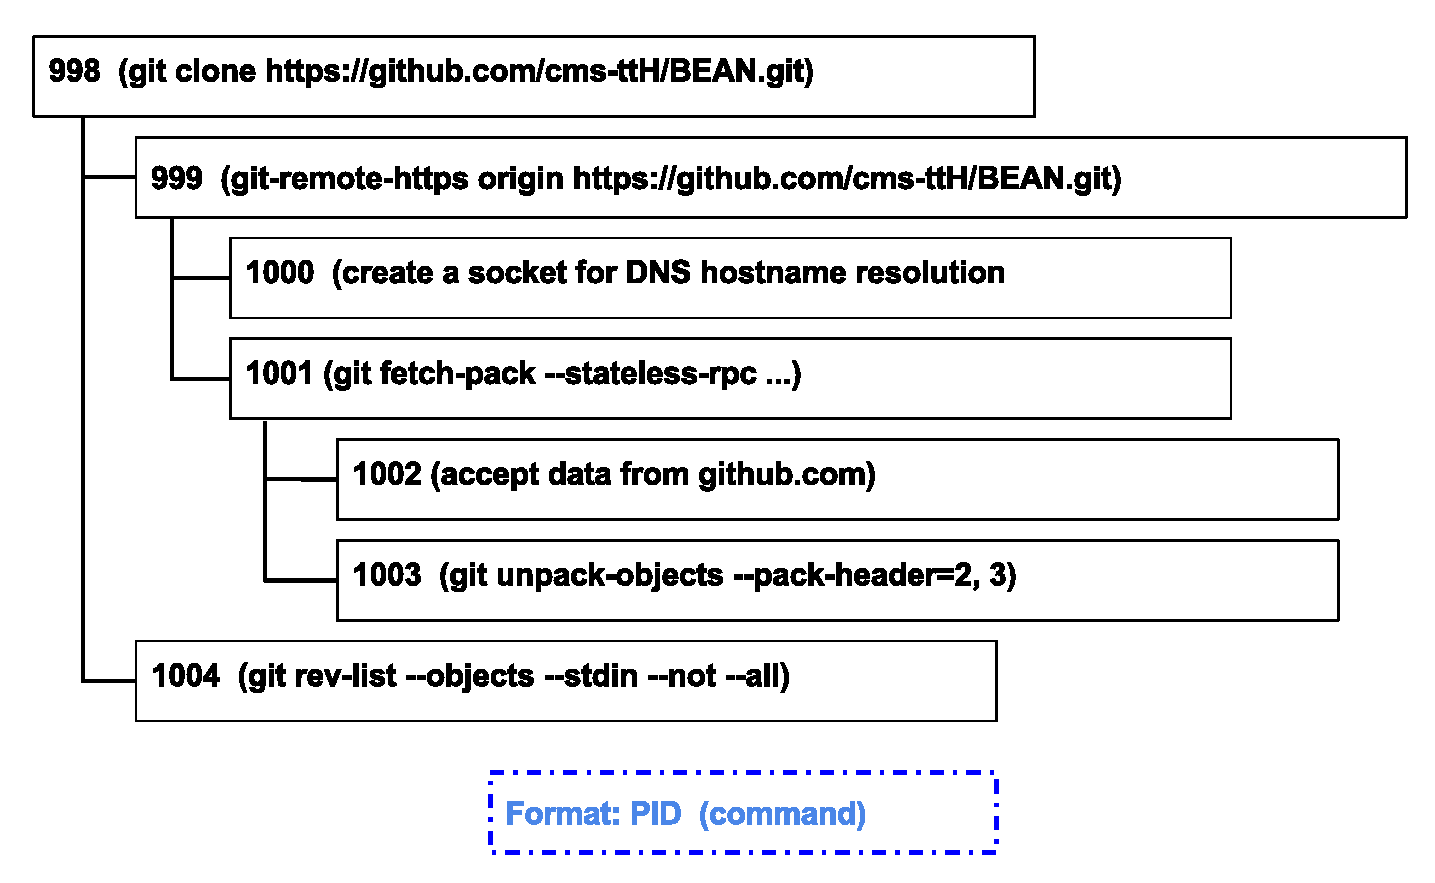
\includegraphics[width=.6\textwidth]{git-syscall.eps}
%\caption{Exec Syscalls of a git command}
%\label{fig:git-syscall}
%\end{figure}
%
%\begin{figure}
%\centering
%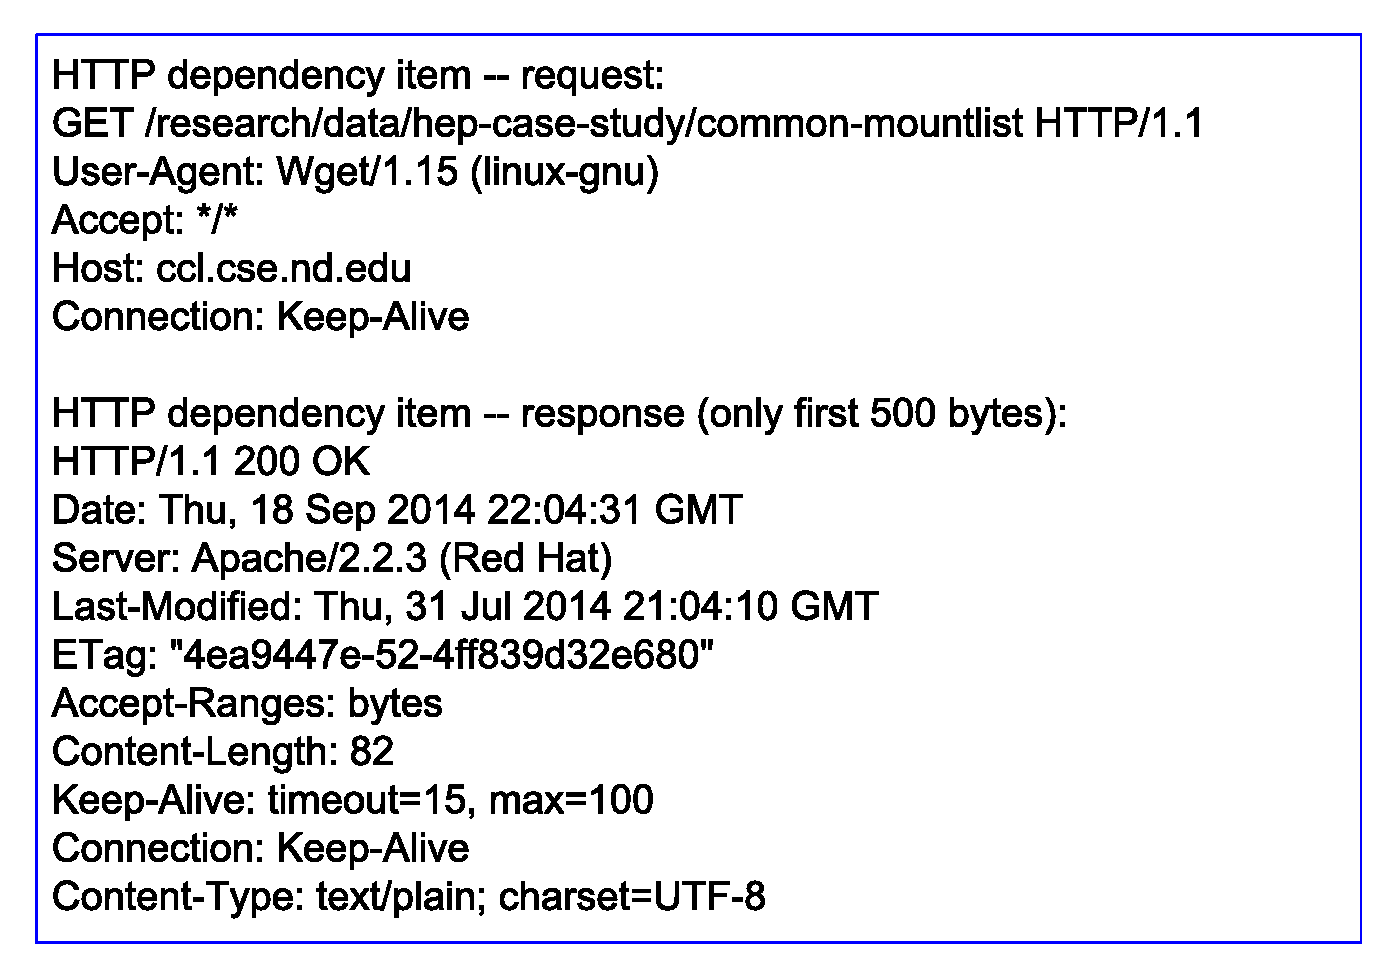
\includegraphics[width=.6\textwidth]{http_packet.eps}
%\caption{HTTP Request and Response}
%\label{fig:http_packet}
%\end{figure}
%
%\begin{figure}
%\centering
%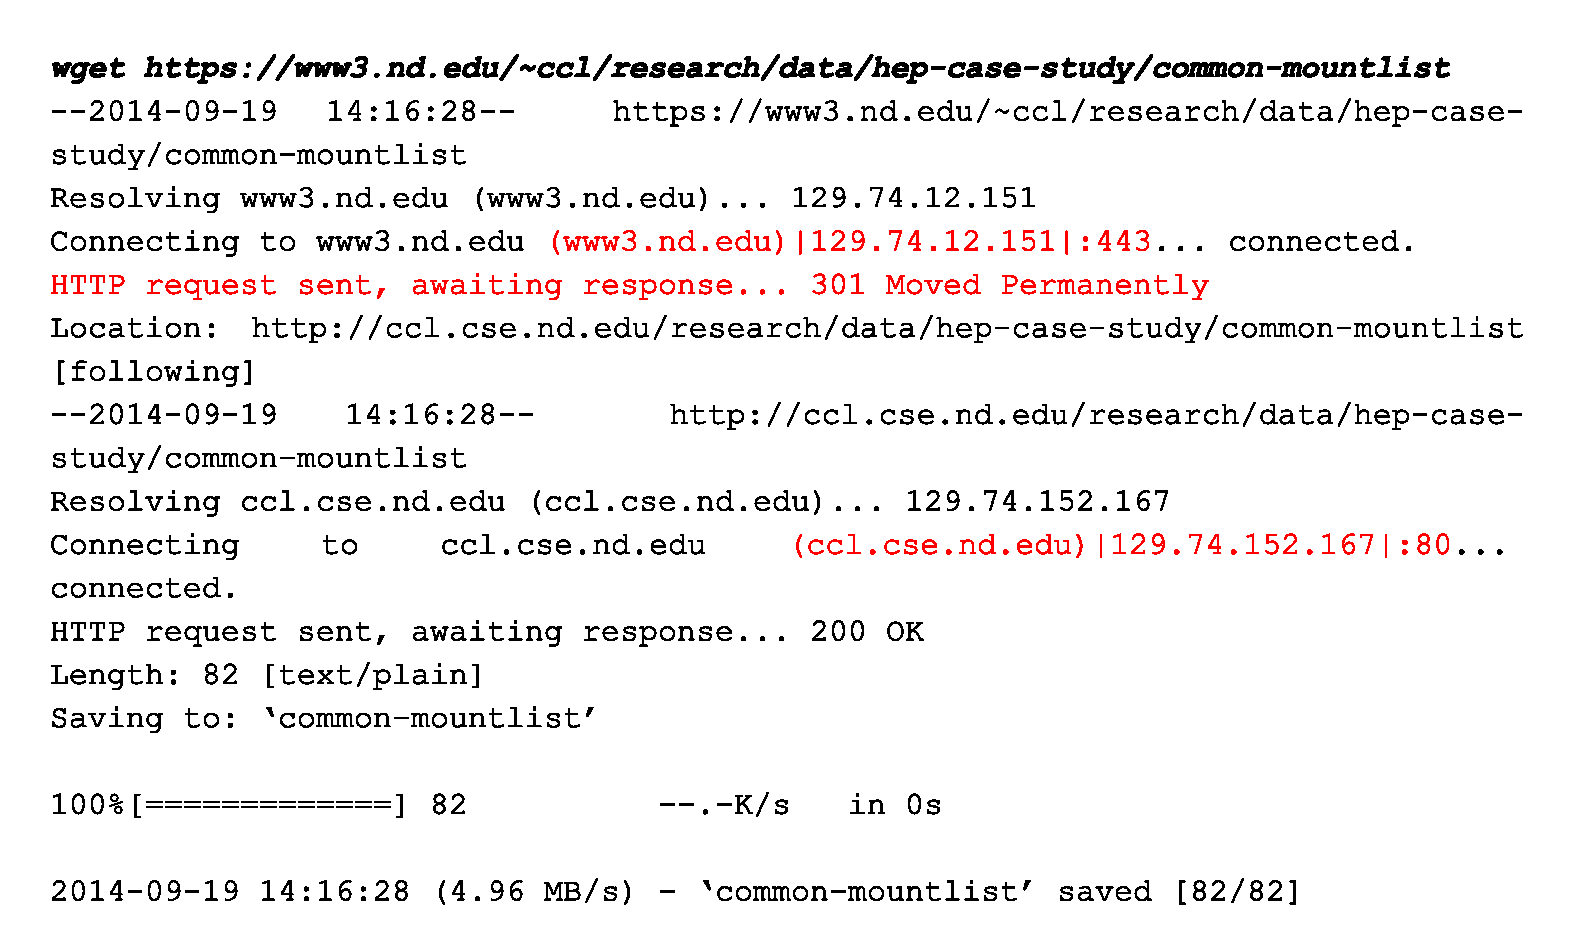
\includegraphics[width=.6\textwidth]{url_redirection.eps}
%\caption{An Example of URL Redirection}
%\label{fig:url_redirection}
%\end{figure}
%
%All the dependencies of one program can be divided into three categories: local file system (e.g., /usr, /lib and /lib64), remote file systems which can be mounted as local directories (e.g., /cvmfs and /hdfs), and other remote network dependencies (e.g. http, https and ssh).
%Through utilizing ptrace to trap each file-relevant system call used by a program, the first two categories of dependencies can be collected. 
%Motivation of tracking network dependencies: Linkrot is a common and great threat to the preservation of scientific applications. A URL which works normally today may be unavailable permanently. A method which can help the scientists figure out all the network dependencies of their applications provides the chance to evaluate the stability of each network dependencies and preserve the unstable network resources before linkrot happens.
%One direct solution to track the third category of dependencies is to utilize ptrace to check each exec system call used by a program and record each network-relevant executable and its parameters. However, an executable may create one or more child processes to finish some tasks, and a child process may create their own children processes. Figure~\ref{fig:git-syscall} shows all the processes created by a git command. A process with PID 998 is created to clone a remote git repository into local machine, which totally has 6 child processes. Moreover, a network-relevant executable name collection is necessary to identify network dependencies. The diversity of network-relevant executables and the large process tree generated for a network executable make this solution infeasible.
%
%Another solution to track network dependencies is to track the network sockets. The user process communicates with the network protocol stacks in the kernel through the network socket layer user interface on Linux. From the process tree shown in the above figure, the process with PID 1000 responds to create a socket, connect to a DNS server, send a DNS request packet to the DNS server and receive a DNS response packet from the DNS server. The information gained from the network socket tracking can be divided into three categories.
%\begin{itemize}
%\item The information of network sockets used to communicate with remote network dependences (through socket and connect system calls) can be used to figure out the port number, service name (such as, http, https, and ssh), socket type (stream and datagram),  and the domain type (inet and inet6). 
%\item The contents of DNS packets can be used to figure out the hostname and IP address of each remote network dependency. 
%\item As for applications based on http protocol, all the http requests and responses can be seen, as shown in Figure~\ref{fig:http_packet}. However, as for applications based on https and ssh which encrypt network data using TLS/SSL, tracking network data on the socket level can only see the encrypted data. 
%\end{itemize}
%
%The results of tracking network sockets used by a program involves two categories of network resource redirections, dns-level hostname redirection and website-level url redirection. 
%\begin{itemize}
%\item dns-level hostname redirection: Each DNS packet includes five parts, header, question, answer, authority, and additional. A DNS response packet with the type CNAME has multiple answers. For example, the DNS response packet which tries to resolve {\tt www3.nd.edu} includes two answers. The first answer provides an alias of {\tt www3.nd.edu}, {\tt www-vip.cc.nd.edu}, and the second answer maps the alias to the IP address. 
%{\tt www3.nd.edu} CNAME {\tt www-vip.cc.nd.edu}
%{\tt www-vip.cc.nd.edu} A {\tt 129.74.12.151}
%The CNAME-type DNS packets leave us a question, among the hostname used by the user, the alias(es), the IP address, what should we preserve?
%\item website-level url redirection: Website-level url redirection happens when a website updates its location and still want their old users access their resources using the old url. Figure~\ref{fig:url_redirection} illustrates the url redirection between {\tt \url{www3.nd.edu/~ccl}} and {\tt ccl.cse.nd.edu}. Except for the difference of hostnames, the application layer protocols used by the old-version website and the new-version website is also different: the old website provides services through the https protocol, while the new website provides services through the http protocol. 
%\end{itemize}
%
%The usage of https protocol makes detecting of website-level url redirections through tracking system calls more difficulty and even impossible. All the application data will be encrypted at presentation layer through the TLS/SSL protocol, which is initialized at the session layer and works at the presentation layer.

